\section{Referencia de la Clase Cobro\-View}
\label{classCobroView}\index{CobroView@{CobroView}}
Administra la ventana de con los datos de un cobro.  


{\tt \#include $<$cobroview.h$>$}

Diagrama de herencias de Cobro\-View\begin{figure}[H]
\begin{center}
\leavevmode
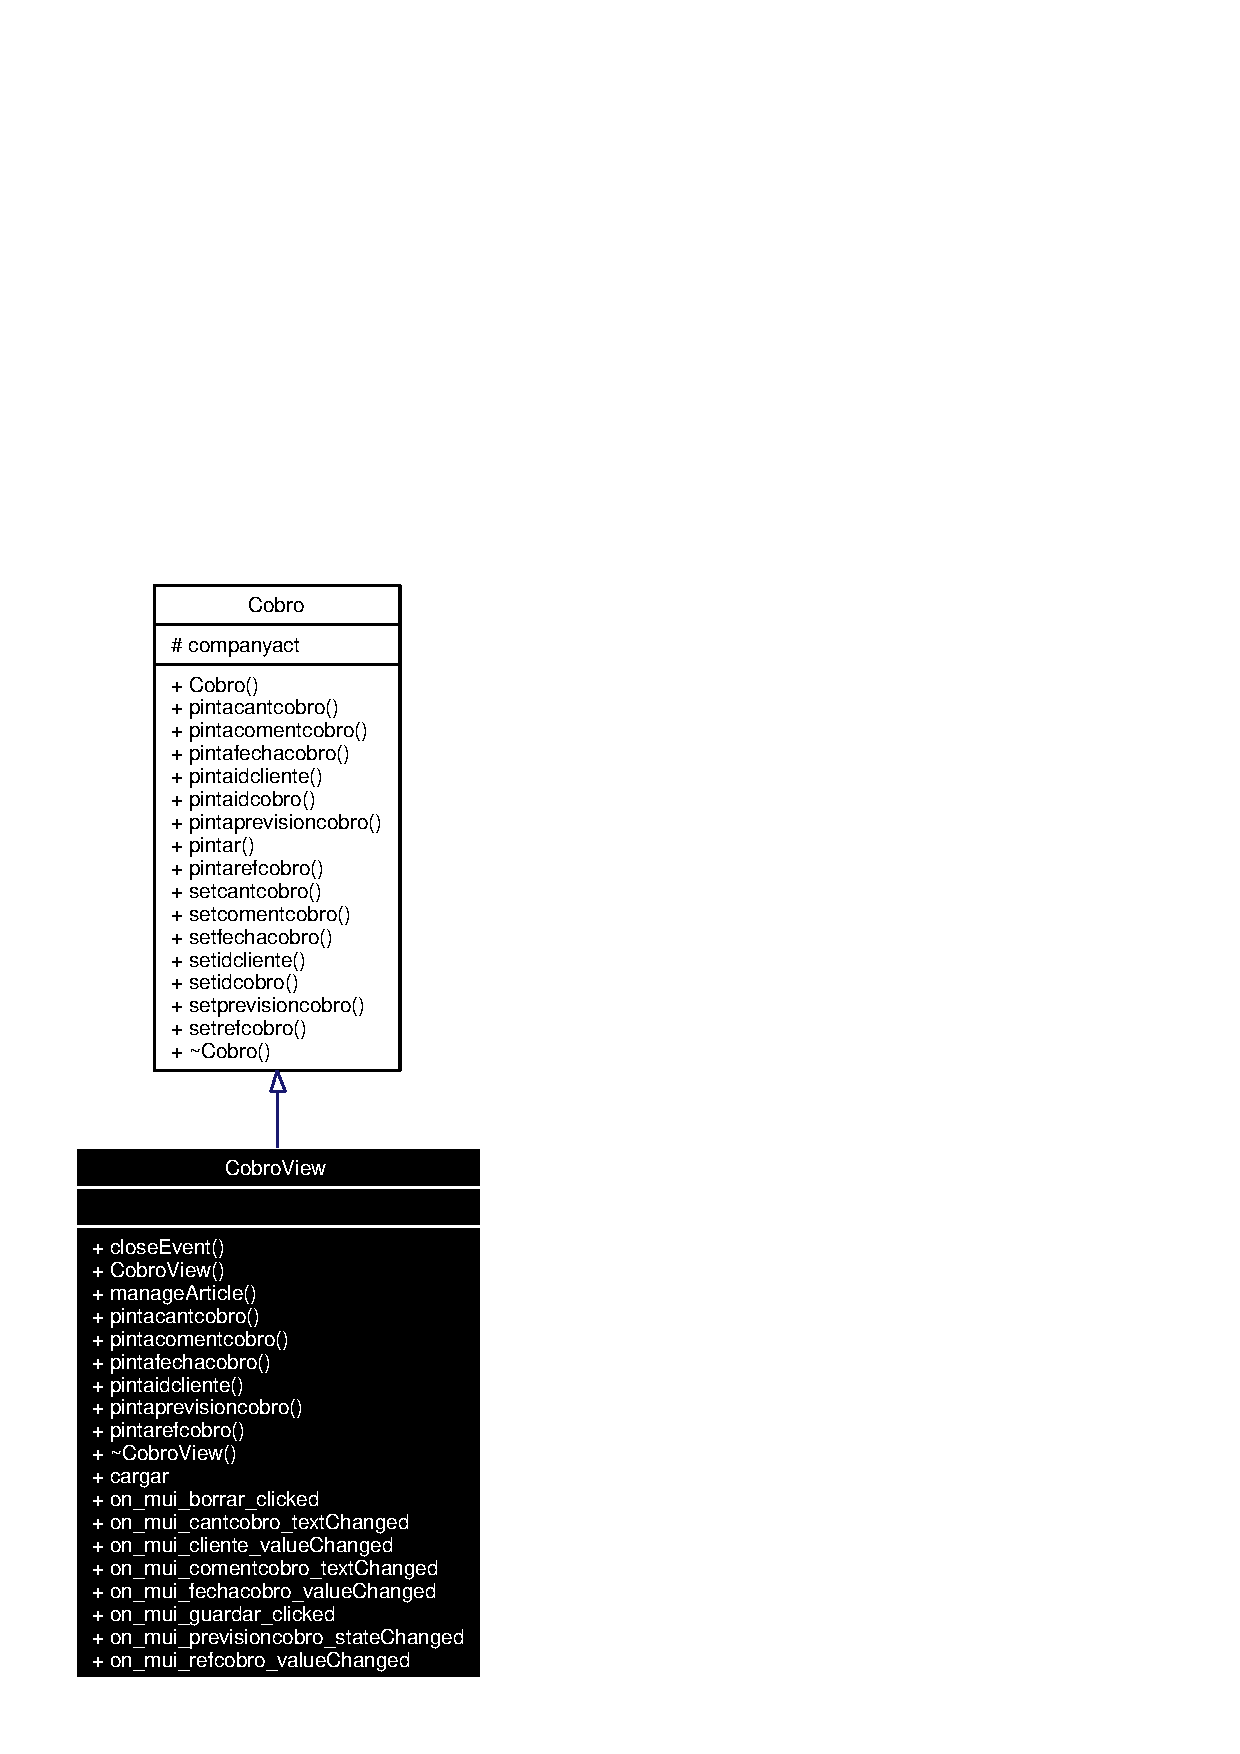
\includegraphics[width=115pt]{classCobroView__inherit__graph}
\end{center}
\end{figure}
Diagrama de colaboraci\'{o}n para Cobro\-View:\begin{figure}[H]
\begin{center}
\leavevmode
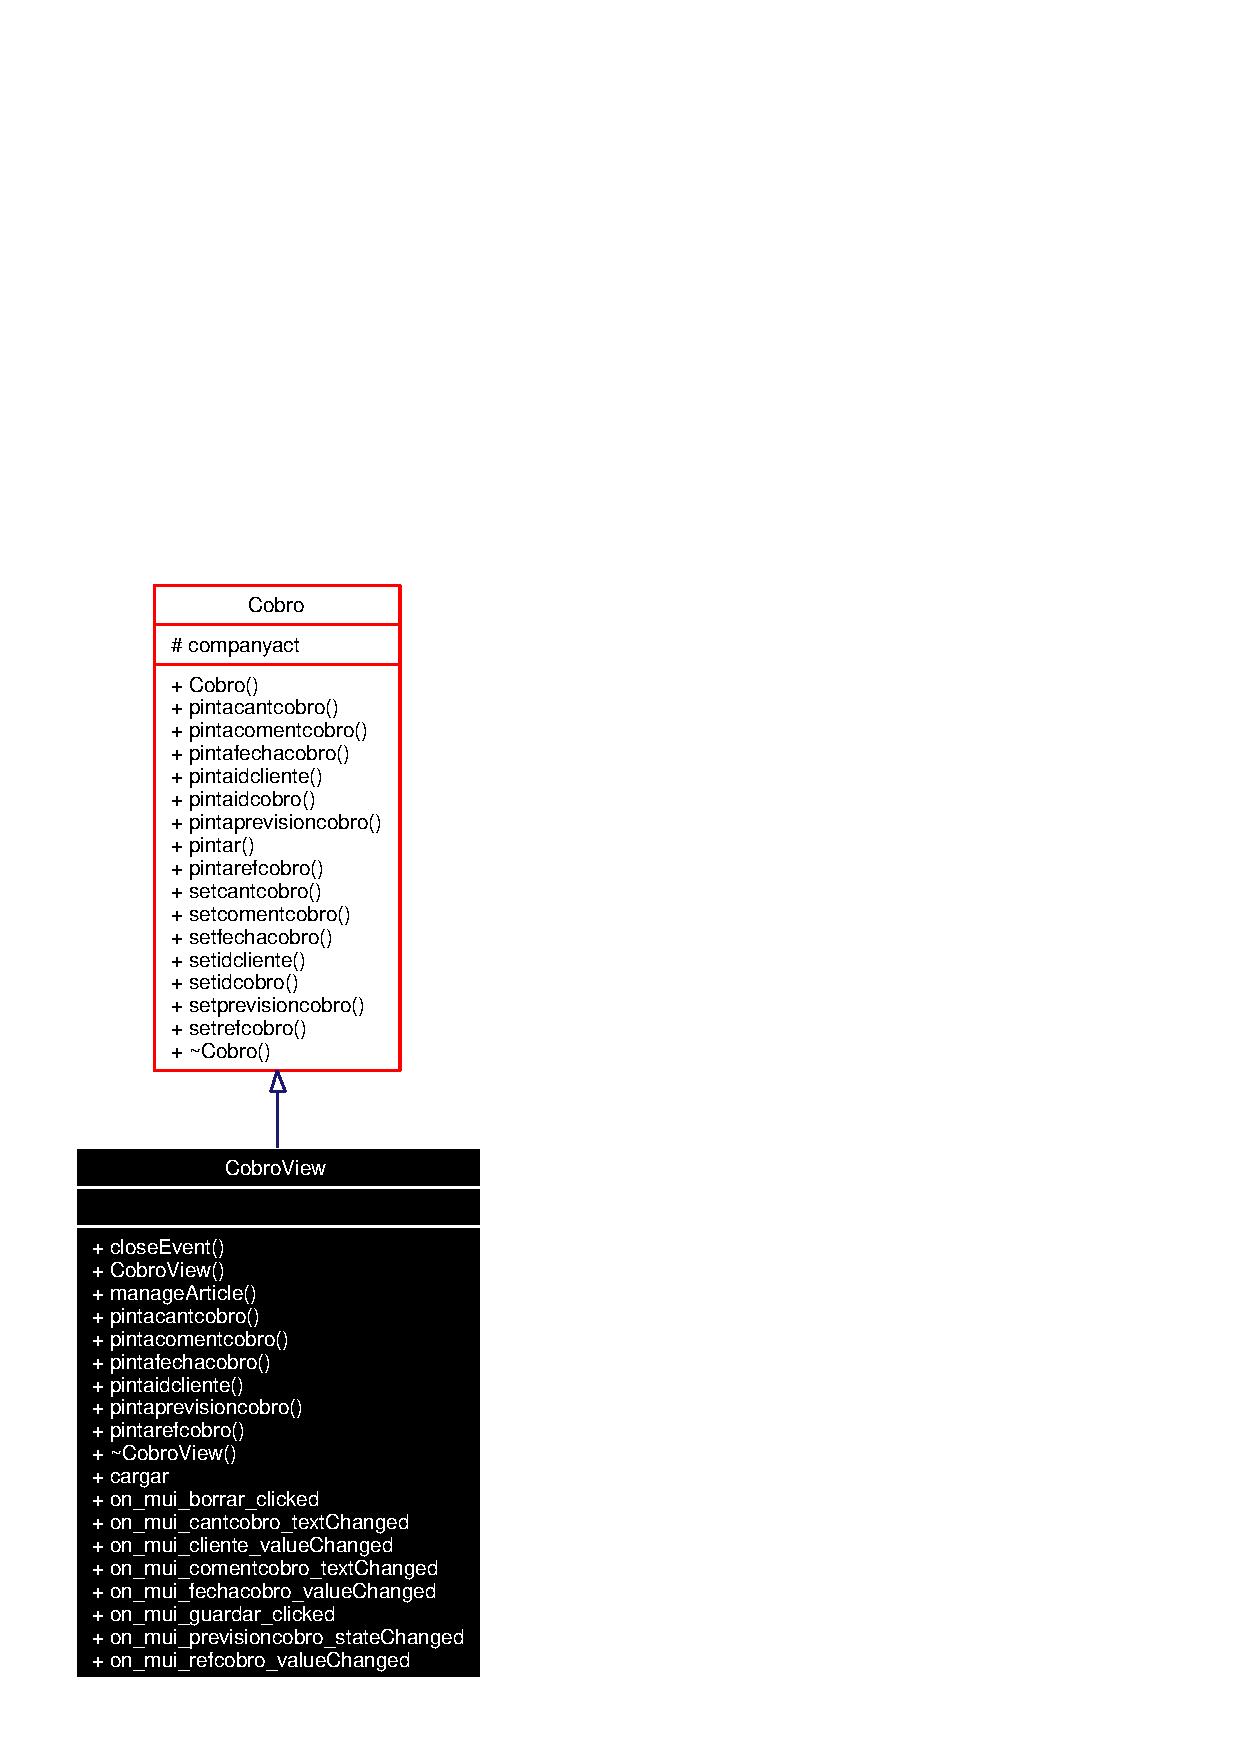
\includegraphics[width=115pt]{classCobroView__coll__graph}
\end{center}
\end{figure}
\subsection*{Slots p\'{u}blicos}
\begin{CompactItemize}
\item 
virtual int {\bf cargar} (QString id)\label{classCobroView_i0}

\item 
virtual void {\bf on\_\-mui\_\-borrar\_\-clicked} ()\label{classCobroView_i1}

\item 
virtual void {\bf on\_\-mui\_\-cantcobro\_\-text\-Changed} (const QString \&str)\label{classCobroView_i2}

\item 
virtual void {\bf on\_\-mui\_\-cliente\_\-value\-Changed} (QString id)\label{classCobroView_i3}

\item 
virtual void {\bf on\_\-mui\_\-comentcobro\_\-text\-Changed} (const QString \&str)\label{classCobroView_i4}

\item 
virtual void {\bf on\_\-mui\_\-fechacobro\_\-value\-Changed} (QString id)\label{classCobroView_i5}

\item 
virtual void {\bf on\_\-mui\_\-guardar\_\-clicked} ()\label{classCobroView_i6}

\item 
virtual void {\bf on\_\-mui\_\-previsioncobro\_\-state\-Changed} (int i)\label{classCobroView_i7}

\item 
virtual void {\bf on\_\-mui\_\-refcobro\_\-value\-Changed} (const QString \&str)\label{classCobroView_i8}

\end{CompactItemize}
\subsection*{M\'{e}todos p\'{u}blicos}
\begin{CompactItemize}
\item 
void {\bf close\-Event} (QClose\-Event $\ast$)\label{classCobroView_a0}

\item 
{\bf Cobro\-View} ({\bf company} $\ast$, QWidget $\ast$)
\item 
void {\bf manage\-Article} (int)\label{classCobroView_a2}

\item 
void {\bf pintacantcobro} (QString id)\label{classCobroView_a3}

\item 
void {\bf pintacomentcobro} (QString id)\label{classCobroView_a4}

\item 
void {\bf pintafechacobro} (QString id)\label{classCobroView_a5}

\item 
void {\bf pintaidcliente} (QString id)\label{classCobroView_a6}

\item 
void {\bf pintaprevisioncobro} (QString id)\label{classCobroView_a7}

\item 
void {\bf pintarefcobro} (QString id)\label{classCobroView_a8}

\end{CompactItemize}


\subsection{Descripci\'{o}n detallada}
Administra la ventana de con los datos de un cobro. 



\subsection{Documentaci\'{o}n del constructor y destructor}
\index{CobroView@{Cobro\-View}!CobroView@{CobroView}}
\index{CobroView@{CobroView}!CobroView@{Cobro\-View}}
\subsubsection{\setlength{\rightskip}{0pt plus 5cm}Cobro\-View::Cobro\-View ({\bf company} $\ast$ {\em comp}, QWidget $\ast$ {\em parent})}\label{classCobroView_a1}


Usurpamos la identidad de mlist y ponemos nuestro propio widget con sus cosillas. 

La documentaci\'{o}n para esta clase fu\'{e} generada a partir de los siguientes archivos:\begin{CompactItemize}
\item 
cobroview.h\item 
cobroview.cpp\end{CompactItemize}
